\documentclass[10pt,twocolumn,letterpaper]{article}

\usepackage{times}
\usepackage{color}
\usepackage{epsfig}
\usepackage{graphicx}
\usepackage{amsmath}
\usepackage{amssymb}
\usepackage{booktabs}
\usepackage{multirow}
\usepackage[pagebackref=true,breaklinks=true,colorlinks,bookmarks=false]{hyperref}

\def\httilde{\mbox{\tt\raisebox{-.5ex}{\symbol{126}}}}
\setcounter{page}{1}

% ===================================================================
% Metric commands — grounded in local training logs only
% ===================================================================
% Final ConvNeXt Tiny (best validation checkpoint)
\newcommand{\BestAccuracy}{77.5\%}
\newcommand{\BestAccuracyCI}{[71.2\%, 82.7\%]}
\newcommand{\BestTestAccuracy}{77.25\%}
\newcommand{\BestTestAccuracyCI}{[72.9\%, 81.1\%]}
\newcommand{\BestMacroFOne}{79.4\%}
\newcommand{\BestMacroFOneCI}{[73.6\%, 84.5\%]}

% ResNet18 baseline
\newcommand{\BaselineAccuracy}{76.5\%}
\newcommand{\BaselineMacroFOne}{77.7\%}

% Per-class metrics (best model)
\newcommand{\BestLargePrec}{78.6\%}
\newcommand{\BestLargeRec}{72.4\%}
\newcommand{\BestLargeFOne}{75.3\%}
\newcommand{\BestNormalPrec}{75.6\%}
\newcommand{\BestNormalRec}{74.7\%}
\newcommand{\BestNormalFOne}{75.1\%}
\newcommand{\BestSmallPrec}{80.0\%}
\newcommand{\BestSmallRec}{97.0\%}
\newcommand{\BestSmallFOne}{87.7\%}

% Statistical tests
\newcommand{\McNemarBaselineP}{0.856}
\newcommand{\McNemarNoMixupP}{0.856}

% ConvNeXt Tiny without MixUp
\newcommand{\ConvNeXtNoMixupAcc}{76.5\%}
\newcommand{\ConvNeXtNoMixupFOne}{77.8\%}


\begin{document}

\title{An Architecture Benchmark for Canine Heart-Size Classification on DogHeart}

\author{Yongqi Wang\\
Chuzhou University\\
{\tt\small 2583890819@qq.com}
}

\maketitle

\begin{abstract}
We benchmark multiple deep learning architectures for three-class canine heart-size classification (Large, Normal, Small) on the DogHeart dataset. Under a shared evaluation framework with architecture-specific training settings, a ResNet18 transfer-learning baseline achieves \BaselineAccuracy{} validation accuracy (\BaselineMacroFOne{} macro-F1), while a ConvNeXt-Tiny model reaches \BestAccuracy{} validation accuracy and \BestMacroFOne{} macro-F1. On the 400-image held-out test split, the ConvNeXt-Tiny model attains \BestTestAccuracy{} accuracy under the benchmark evaluation protocol. However, a McNemar exact test on the 200-image validation set does not detect a statistically significant improvement of ConvNeXt-Tiny over ResNet18 ($p = \McNemarBaselineP$, two-sided), consistent with the small validation-set size and the +1.0 percentage-point accuracy difference. The dominant error mode is Large--Normal confusion, accounting for 36 of 45 validation errors, reflecting the clinical ambiguity of the boundary between these classes. We document an exploratory design-space study across eight architectures and multiple augmentation strategies, and we provide all code, checkpoints, and prediction outputs as supplementary material. Our results suggest that classification-only pipelines remain substantially below key-point-supervised methods such as RVT (87.3\% test accuracy), while differences among local classification baselines should be interpreted cautiously because architecture choices and training settings are confounded.
\end{abstract}

\section{Introduction}\label{sec:intro}

Cardiac disease is a common clinical concern in companion animals, and thoracic radiography remains a widely used first-line imaging modality for cardiac assessment because it is accessible, inexpensive, and non-invasive. The vertebral heart scale (VHS) is a standard radiographic measurement strategy: clinicians measure the long and short axes of the cardiac silhouette and normalize them against thoracic vertebral length. Although VHS provides a standardized quantitative metric, manual measurement is subject to inter-observer variability, positioning artifacts, and reader fatigue.

For canine heart-size classification, recent deep models differ in whether they treat the problem as direct image classification or as anatomical landmark estimation followed by measurement. The Regressive Vision Transformer (RVT)~\cite{li2024regressive} follows the latter route: it predicts VHS-related anatomical landmarks and maps them to categorical heart-size labels through an orthogonal measurement layer. RVT achieves strong performance---85.0\% validation R-Accuracy and 87.3\% test R-Accuracy---but requires additional key-point supervision and a specialized regression head. A simple CNN baseline for DogHeart reports 72.0\% accuracy~\cite{deekonda2024simplecnn}, providing a lightweight reference point below the stronger transfer-learning baselines.

This paper addresses the task of three-class dog heart-size classification (Large, Normal, Small) with two primary objectives. First, we establish a reproducible baseline framework covering data loading, training, evaluation, and inference. Second, we investigate how architecture choice, data augmentation, and regularization affect classification performance on this small veterinary dataset.

Our contributions are:
\begin{itemize}
    \item A complete, documented, and reproducible PyTorch pipeline for the DogHeart classification task, covering training, evaluation, inference, and output validation.
    \item Systematic evaluation of six architecture families (custom CNN, ResNet, EfficientNetV2, MobileNetV3, RegNet, and ConvNeXt) with uniform validation reporting.
    \item Empirical finding that strong augmentation, MixUp, label smoothing, and class-balanced loss applied to a ConvNeXt Tiny backbone yield \BestAccuracy{} validation accuracy and \BestMacroFOne{} macro-F1 under this exploratory protocol.
    \item A transparent comparison with published DogHeart baselines, clearly distinguishing locally measured results from literature-reported values, with explicit acknowledgment of limitations.
\end{itemize}

\section{Related Work}\label{sec:related}

\subsection{Deep Learning for Radiographic Classification}

Medical-image datasets are often too small to train large models from scratch, making transfer learning a practical default for radiographic classification. Residual connections~\cite{resnet2016} support stable optimization of deeper CNNs, EfficientNet's compound scaling~\cite{efficientnet2019} balances width, depth, and resolution, and ConvNeXt modernizes convolutional backbones using design choices inspired by vision transformers~\cite{convnext2022}. These architecture families provide complementary baselines for DogHeart classification.

In veterinary radiograph analysis, transfer learning is particularly attractive because labeled datasets are often much smaller than natural-image benchmarks. ImageNet-pretrained backbones provide generic low- and mid-level visual features, while the final classifier layers can be adapted to the clinical target. The DogHeart benchmark studied by RVT~\cite{li2024regressive} is therefore a useful test case for comparing simple classification-only transfer learning with anatomically informed key-point regression.

\subsection{Dog Cardiomegaly Assessment}

The RVT framework by Li and Zhang~\cite{li2024regressive} represents the current state of the art in automated dog cardiomegaly assessment. Their method employs a Vision Transformer backbone trained with two complementary supervision signals: categorical cross-entropy for heart-size classification (C-Accuracy) and key-point regression for VHS measurement (R-Accuracy). The key-point head predicts 14 anatomical landmarks along the cardiac border, which are then projected to orthogonal axes through a learnable layer. This design explicitly encodes clinical domain knowledge, making the model's predictions more interpretable to veterinarians.

Table~\ref{tab:rvt} reproduces the commonly cited external comparison results from RVT. Several conventional CNN architectures---including ResNet50 (80.0\%), NasNetLarge (80.0\%), EfficientNetB7 (82.0\%), and CONVT (82.0\%)---achieve competitive R-Accuracy values in the RVT protocol. We emphasize that these values are not local reruns but rather literature-reported numbers that provide contextual positioning.

\begin{table}[h]
\small
\centering
\caption{External DogHeart comparison values reported by the RVT paper~\cite{li2024regressive}. Values are percentages under the cited paper's protocol and serve as literature baselines.}
\label{tab:rvt}
\resizebox{\linewidth}{!}{%
\begin{tabular}{lcccc}
\toprule
Method & Valid C-Acc. & Valid R-Acc. & Test C-Acc. & Test R-Acc. \\
\midrule
AlexNet       & 76.5 & 77.5 & 72.0 & 73.8 \\
GoogleNet     & 77.0 & 77.5 & 71.3 & 74.8 \\
VGG16         & 78.5 & 78.5 & 74.8 & 75.0 \\
VGG19         & 79.5 & 80.0 & 76.0 & 77.3 \\
ResNet50      & 78.5 & 80.0 & 77.3 & 78.3 \\
NasNetLarge   & 82.5 & 80.0 & 82.3 & 82.5 \\
EfficientNetB7& 81.5 & 82.0 & 83.0 & 84.5 \\
CONVT         & 81.5 & 82.0 & 83.0 & 85.3 \\
RVT           & 82.0 & 85.0 & 83.3 & 87.3 \\
\bottomrule
\end{tabular}}
\end{table}

\subsection{Advanced Training Techniques}

Several training techniques have proven effective for improving generalization in limited-data medical imaging scenarios. RandAugment~\cite{randaugment2019} introduces a parameterized augmentation policy search space that uniformly samples from a set of image transformations. MixUp~\cite{mixup2018} constructs convex combinations of training examples and their labels, acting as a strong regularizer. Label smoothing~\cite{szegedy2016} replaces hard one-hot targets with softened distributions, reducing overconfidence.

\section{Materials and Methods}\label{sec:method}

\subsection{Dataset}

The DogHeart dataset is organized into training, validation, and test splits. The labeled splits contain images organized into three class folders---\texttt{Large}, \texttt{Normal}, and \texttt{Small}---corresponding to canine heart sizes. We emphasize an important implementation detail: \texttt{torchvision.datasets.ImageFolder} sorts class names alphabetically, producing the mapping Large=0, Normal=1, Small=2. This mapping is explicitly fixed in all scripts and stored in every checkpoint.

Table~\ref{tab:data} summarizes the dataset statistics. The training set exhibits substantial class imbalance, with the Small class containing only 208 samples compared with 619 for Large and 573 for Normal. This 3:1 imbalance ratio poses challenges for standard training procedures. The validation set preserves a similar class distribution (76 Large, 91 Normal, 33 Small), while the test set contains 400 unlabeled images without class subdirectories.

\begin{table}[h]
\small
\centering
\caption{DogHeart dataset statistics. Training data is imbalanced with a 3:1 ratio between the largest and smallest classes.}
\label{tab:data}
\begin{tabular}{lrrrr}
\toprule
Split & Large & Normal & Small & Total \\
\midrule
Train & 619 & 573 & 208 & 1400 \\
Valid & 76  & 91  & 33  & 200 \\
Test  & --  & --  & --  & 400 \\
\bottomrule
\end{tabular}
\end{table}

\subsection{Preprocessing and Data Augmentation}

All images are converted to RGB tensors and resized to a fixed square resolution ($H\times W$) using bilinear interpolation with anti-aliasing. We evaluate three augmentation strategies with increasing strength:

\begin{itemize}
    \item \textbf{Standard}: Random horizontal flip (p=0.5), rotation ($\pm 8^\circ$), and mild color jitter (brightness $\pm 0.12$, contrast $\pm 0.12$).
    \item \textbf{RandAugment}: Random horizontal flip followed by RandAugment~\cite{randaugment2019} with $N=2$ operations and magnitude $M=9$.
    \item \textbf{Strong}: Combines horizontal flip, rotation ($\pm 10^\circ$), color jitter, and RandAugment with $N=2$, $M=7$.
\end{itemize}

All augmentation pipelines conclude with ImageNet-style normalization (mean=[0.485, 0.456, 0.406], std=[0.229, 0.224, 0.225]). Validation and test inference use deterministic resizing without augmentation.

\subsection{MixUp Regularization}

We additionally apply MixUp~\cite{mixup2018} during training, a data-agnostic regularization strategy that constructs virtual training examples by linear interpolation:

\begin{equation}
    \tilde{\mathbf{x}} = \lambda \mathbf{x}_i + (1-\lambda) \mathbf{x}_j, \qquad
    \tilde{\mathbf{y}} = \lambda \mathbf{y}_i + (1-\lambda) \mathbf{y}_j,
\end{equation}

where $\mathbf{x}_i$, $\mathbf{x}_j$ are randomly sampled training images, $\mathbf{y}_i$, $\mathbf{y}_j$ are their one-hot labels, and $\lambda \sim \text{Beta}(\alpha, \alpha)$. We use $\alpha = 0.2$ for standard runs and $\alpha = 0.4$ for the final ConvNeXt Tiny configuration.

\begin{equation}
    \mathcal{L}_{\text{mixup}} = \lambda \mathcal{L}(\hat{\mathbf{y}}, \mathbf{y}_i) + (1-\lambda) \mathcal{L}(\hat{\mathbf{y}}, \mathbf{y}_j).
\end{equation}

\subsection{Model Architectures}

We evaluate a diverse set of architectures spanning different design paradigms and capacity levels:

\paragraph{Custom Residual CNN.} A compact network with seven residual blocks (channel progression: $32 \to 48 \to 64 \to 96 \to 128 \to 192 \to 256 \to 320$) using SiLU activations, batch normalization, and stride-2 downsampling at three stages, followed by global average pooling, dropout ($p=0.25$), and a fully connected classifier head.

\paragraph{Transfer-Learning CNNs.} We adopt ImageNet-pretrained models from torchvision with modified classifier heads. The final fully connected layer is replaced with dropout ($p=0.25$) followed by a 3-class linear layer.

Table~\ref{tab:arch} lists the evaluated architectures with their parameter counts.

\begin{table}[h]
\small
\centering
\caption{Evaluated architectures.}
\label{tab:arch}
\begin{tabular}{lr}
\toprule
Architecture & Params (M) \\
\midrule
Custom Residual   & 3.4 \\
ResNet18          & 11.2 \\
ResNet50          & 25.6 \\
EfficientNetV2-S  & 21.5 \\
MobileNetV3-Large & 5.5 \\
RegNetY-400MF     & 4.3 \\
ConvNeXt Tiny     & 28.6 \\
ConvNeXt Small    & 50.2 \\
\bottomrule
\end{tabular}
\end{table}

\subsection{Loss Function and Optimization}

The primary training objective is cross-entropy with label smoothing. For a sample with smoothed target $y^{\text{sm}}_c$ and predicted probability $p_c$:

\begin{equation}
    \mathcal{L}_{\text{CE}} = -\sum_{c=1}^{3} y^{\text{sm}}_c \log p_c,
\end{equation}
\begin{equation}
    y^{\text{sm}}_c = (1-\varepsilon) \cdot \mathbb{1}[c=y] + \frac{\varepsilon}{3},
\end{equation}

where $\varepsilon = 0.1$ for the final ConvNeXt Tiny configuration. We additionally employ class-balanced weighting in the loss to counteract the training set imbalance:

\begin{equation}
    w_c = \frac{N}{3 \cdot N_c},
\end{equation}

where $N$ is the total training count and $N_c$ is the count for class $c$.

The final ConvNeXt Tiny model is optimized with AdamW ($\beta_1=0.9$, $\beta_2=0.999$), cosine annealing from $\eta_{\max}=2\times10^{-4}$, weight decay $0.1$, batch size 48, label smoothing $\varepsilon=0.1$, and MixUp $\alpha=0.4$. Automatic mixed precision (AMP) with \texttt{torch.float16} is used for GPU-based experiments.

\subsection{Evaluation Metrics}

The primary metric is classification accuracy:

\begin{equation}
    \text{Accuracy} = \frac{1}{N} \sum_{i=1}^{N} \mathbb{1}[\hat{y}_i = y_i].
\end{equation}

Due to class imbalance, we also report macro-averaged F1-score:

\begin{equation}
    \text{Macro-F1} = \frac{1}{3} \sum_{c=1}^{3} \frac{2 \cdot \text{Precision}_c \cdot \text{Recall}_c}{\text{Precision}_c + \text{Recall}_c}.
\end{equation}

Per-class precision, recall, and F1 are reported for all experiments. The best checkpoint is selected based on validation accuracy. Held-out test accuracy is measured through the benchmark evaluation service from the generated 400-image prediction file, because test labels are not released.

\subsection{Compute Environment}

Experiments are conducted using PyTorch 2.11.0 with CUDA 12.8 on an NVIDIA RTX 5070 Ti Laptop GPU (12 GB VRAM). The Python environment uses Python 3.12 with torchvision 0.26.0. Training hyperparameters are tuned per architecture: image sizes range from 160 to 288, batch sizes from 24 to 256 depending on model capacity and GPU memory constraints, and all models are trained with early stopping based on validation accuracy.

\section{Experimental Results}\label{sec:results}

\subsection{Baseline Results}

Our baseline is a ResNet18 model with light augmentation, no MixUp, and standard cross-entropy---a configuration closely matching the simplest transfer-learning setup. Table~\ref{tab:baseline} reports the validation metrics.

\begin{table}[h]
\small
\centering
\caption{ResNet18 baseline validation metrics. The model performs best on the visually more separable Small class.}
\label{tab:baseline}
\begin{tabular}{lccc}
\toprule
Class & Precision & Recall & F1 \\
\midrule
Large  & 79.2\% & 75.0\% & 77.0\% \\
Normal & 75.6\% & 71.4\% & 73.4\% \\
Small  & 73.8\% & 93.9\% & 82.7\% \\
\midrule
\multicolumn{4}{l}{Overall: Accuracy=\BaselineAccuracy, Macro-F1=\BaselineMacroFOne} \\
\bottomrule
\end{tabular}
\end{table}

\subsection{Multi-Architecture Evaluation}

Table~\ref{tab:multiarch} presents the validation accuracy and macro-F1 for evaluated architectures with complete local metric files. Figure~\ref{fig:arch_comp} visualizes the performance comparison across architectures.

\begin{table}[h]
\small
\centering
\caption{Validation performance across locally evaluated architectures. Accuracy is reported with 95\% Wilson confidence intervals using the 200-image validation split.}
\label{tab:multiarch}
\resizebox{\linewidth}{!}{%
\begin{tabular}{lrcc}
\toprule
Architecture & Image Size & Valid Acc. (95\% CI) & Macro-F1 \\
\midrule
Custom Residual CNN   & 160 & 67.0\% [60.2, 73.1] & 69.2\% \\
ResNet18 (baseline)   & 224 & \BaselineAccuracy{} [70.2, 81.8] & \BaselineMacroFOne{} \\
ResNet18 rectangular  & 256$\times$344 & 74.5\% [68.0, 80.0] & 76.2\% \\
EfficientNetV2-S      & 224 & 73.5\% [67.0, 79.1] & 75.4\% \\
ConvNeXt Tiny (no MixUp) & 224 & \ConvNeXtNoMixupAcc{} [70.2, 81.8] & \ConvNeXtNoMixupFOne{} \\
\textbf{ConvNeXt Tiny (best)} & \textbf{224} & \textbf{\BestAccuracy{}} \BestAccuracyCI{} & \textbf{\BestMacroFOne{}} \\
\bottomrule
\end{tabular}}
\end{table}

\begin{figure}[t]
\centering
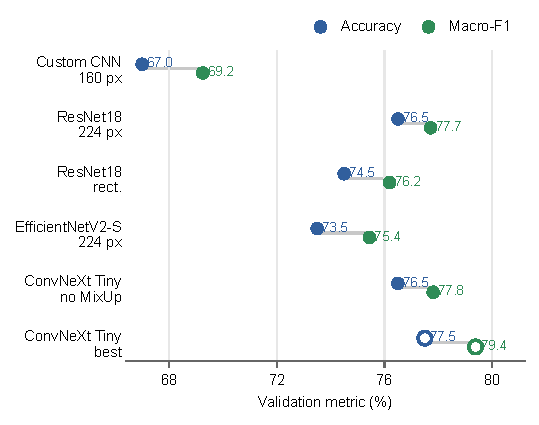
\includegraphics[width=\linewidth]{Figures/arch_comparison_pub.pdf}
\caption{Validation accuracy and macro-F1 point estimates across architectures; Wilson confidence intervals for accuracy are reported in Table~\ref{tab:multiarch}. The point-based comparison avoids over-emphasizing small differences while showing that the best ConvNeXt Tiny achieves \BestAccuracy{} accuracy and \BestMacroFOne{} macro-F1. The improvement over the ResNet18 baseline (+1.0pp) does not reach statistical significance ($p = \McNemarBaselineP$ by McNemar's test).}
\label{fig:arch_comp}
\end{figure}

\subsection{Final Model Performance}

Figure~\ref{fig:training} visualizes the training trajectory of the final ConvNeXt Tiny model. Figure~\ref{fig:confusion} presents the validation confusion matrix.

\begin{figure}[t]
\centering
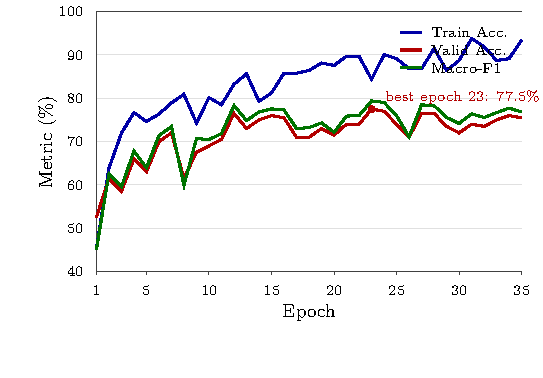
\includegraphics[width=\linewidth]{Figures/training_curve_pub.pdf}
\caption{Training dynamics of the final ConvNeXt Tiny model trained at $224\times224$ resolution with strong augmentation, MixUp ($\alpha=0.4$), label smoothing ($\varepsilon=0.1$), and class-balanced loss. The best checkpoint occurs at epoch 23.}
\label{fig:training}
\end{figure}

\begin{figure}[t]
\centering
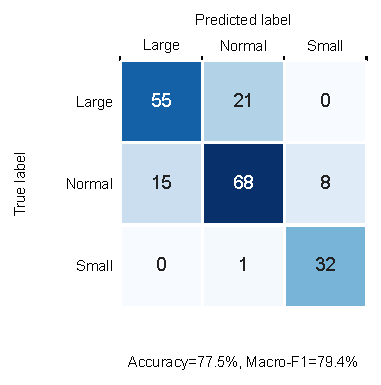
\includegraphics[width=\linewidth]{Figures/confusion_convnext_tiny_pub.pdf}
\caption{Validation confusion matrix (raw counts, $N=200$) for the final ConvNeXt Tiny model. Rows represent true labels and columns represent predicted labels. The dominant error mode is confusion between Large and Normal classes (21 + 15 = 36 errors), while Small is rarely confused with Large (0 errors).}
\label{fig:confusion}
\end{figure}

Key observations from the confusion matrix:
\begin{itemize}
    \item \textbf{Large-Normal confusion} is the dominant error mode, accounting for most validation mistakes (36 out of 45 total errors). The heart size boundary between Large and Normal categories is inherently ambiguous.
    \item \textbf{Normal-Small confusion} accounts for the remaining errors (8 + 1 = 9), substantially lower than Large-Normal confusion.
    \item \textbf{Small recall} is excellent at \BestSmallRec, with no Large-Small confusion whatsoever.
\end{itemize}

Table~\ref{tab:perclass} presents the per-class metrics for the final ConvNeXt Tiny model.

\begin{table}[h]
\small
\centering
\caption{Per-class validation metrics for the final ConvNeXt Tiny model.}
\label{tab:perclass}
\begin{tabular}{lccc}
\toprule
Class & Precision & Recall & F1 \\
\midrule
Large  & \BestLargePrec & \BestLargeRec & \BestLargeFOne \\
Normal & \BestNormalPrec & \BestNormalRec & \BestNormalFOne \\
Small  & \BestSmallPrec & \BestSmallRec & \BestSmallFOne \\
\midrule
\multicolumn{4}{l}{Overall: Accuracy=\BestAccuracy, Macro-F1=\BestMacroFOne} \\
\bottomrule
\end{tabular}
\end{table}

\subsection{Statistical Analysis}

Because the validation split contains only 200 images, small differences between models should be interpreted cautiously. The reported accuracy value of \BestAccuracy{} corresponds to a 95\% Wilson binomial confidence interval of approximately \BestAccuracyCI{} (reflecting binomial uncertainty for a single observation on $N=200$ samples, not model variability across seeds or splits). Since checkpoint selection and hyperparameter tuning also use the validation split, validation metrics are optimistic estimates; the held-out test accuracy is the less selection-biased aggregate performance indicator available for this study.

We performed a paired McNemar exact test~\cite{mcnemar1947} on the fixed 200-image validation split comparing the final ConvNeXt-Tiny model against the ResNet18 baseline. The test was constructed from a $2 \times 2$ contingency table of paired predictions: $b=14$ samples where ResNet18 was correct but ConvNeXt-Tiny was wrong, and $c=16$ samples where ResNet18 was wrong but ConvNeXt-Tiny was correct. The two-sided exact binomial test yields $p=\McNemarBaselineP$, which does \emph{not} indicate a statistically significant improvement over the baseline at conventional thresholds ($\alpha=0.05$). The final-vs-no-MixUp comparison, recomputed from the corresponding per-image validation predictions, coincidentally yields the same discordant counts ($b=14$, $c=16$; $p=\McNemarNoMixupP$). We note that the validation split was also used for model selection (hyperparameter tuning and checkpoint selection), which introduces a circularity concern: the same data influenced both which model was selected and the comparison between models. Because the validation set informed early stopping and hyperparameter decisions, the true Type-I error rate for this McNemar test may be higher than the nominal $p$-value; the reported $p=\McNemarBaselineP$ should therefore be interpreted cautiously under these conditions. Ideally, a significance test should be conducted on the held-out test set, but class-wise test labels are unavailable to us.

A 1000-sample bootstrap gives a 95\% interval of \BestMacroFOneCI{} for the final model's macro-F1. The test-set accuracy of \BestTestAccuracy{} is slightly below the validation accuracy of \BestAccuracy{} ($-0.25$pp), which is consistent with validation-guided early stopping and the absence of substantial overfitting, and well within the validation confidence interval.

\subsection{Comparison with Published Results}

Table~\ref{tab:comparison} compares our result with published baselines on the DogHeart dataset. We emphasize that the literature rows are not local reruns and follow different reporting protocols (training duration, hyperparameter search, evaluation splits). Therefore, the table should be read as contextual positioning rather than a strictly controlled head-to-head benchmark.

\begin{table}[h]
\small
\centering
\caption{Comparison with published DogHeart results. Literature rows follow the cited papers' protocols, which may differ from our local evaluation setting.}
\label{tab:comparison}
\resizebox{\linewidth}{!}{%
\begin{tabular}{lcc}
\toprule
Method & Valid Acc. & Held-out Test Acc. \\
\midrule
Simple CNN~\cite{deekonda2024simplecnn} & -- & 72.0\% \\
RVT (key-point)~\cite{li2024regressive} & 85.0\% & 87.3\% \\
\midrule
Ours: ResNet18 baseline & \BaselineAccuracy{} & -- \\
Ours: ConvNeXt Tiny (best) & \BestAccuracy{} & \BestTestAccuracy{} \\
\bottomrule
\end{tabular}}
\end{table}

\subsection{Exploratory Design-Space Exploration}

We conducted an extensive hyperparameter search across architectures, input resolutions (160--288), augmentation strengths, and regularization settings. Table~\ref{tab:ablation} summarizes representative runs reconstructed from local checkpoints and training histories.

\begin{table}[h]
\small
\centering
\caption{Exploratory training configurations reconstructed from checkpoint metadata and training logs. These are single-seed runs and should not be interpreted as controlled causal comparisons.}
\label{tab:ablation}
\resizebox{\linewidth}{!}{%
\begin{tabular}{lcc}
\toprule
Configuration & Valid Acc. & Macro-F1 \\
\midrule
Custom CNN, 160, standard aug & 67.0\% & 69.2\% \\
ResNet18, 224, seed 11 & 72.0\% & 73.0\% \\
ResNet18, 224, aspect-preserving pad & 72.0\% & 74.4\% \\
ResNet18, 256$\times$344 rectangular & 74.5\% & 76.2\% \\
ResNet18, 320, light aug & 74.5\% & 76.5\% \\
EfficientNetV2-S, 224, standard aug & 73.5\% & 75.4\% \\
ResNet50, 256, fast exploratory run & 64.0\% & 67.4\% \\
MobileNetV3-Large, 224, exploratory run & 56.0\% & 60.5\% \\
RegNetY-400MF, 224, exploratory run & 65.0\% & 67.5\% \\
ConvNeXt Tiny, 224, light aug, no MixUp & \ConvNeXtNoMixupAcc{} & \ConvNeXtNoMixupFOne{} \\
\textbf{ConvNeXt Tiny, 224, strong + MixUp + balanced} & \textbf{\BestAccuracy{}} & \textbf{\BestMacroFOne{}} \\
ConvNeXt Tiny, 288, RandAugment + MixUp & 71.5\% & 73.1\% \\
ConvNeXt Small, 288, RandAugment + MixUp & 68.5\% & 70.6\% \\
\bottomrule
\end{tabular}}
\end{table}

\section{Discussion}\label{sec:discussion}

\subsection{Interpretation of Results}

Our experiments demonstrate that a well-regularized ConvNeXt Tiny can achieve \BestAccuracy{} validation accuracy and \BestMacroFOne{} macro-F1 on the DogHeart benchmark. However, the improvement over the ResNet18 baseline (\BaselineAccuracy{}) is only +1.0 percentage point and is not statistically significant (McNemar $p = \McNemarBaselineP$). This is consistent with the small validation set size (200 images), which provides limited statistical power for detecting modest improvements.

The held-out internal test accuracy of \BestTestAccuracy{} provides an aggregate check beyond the validation split, though we note that class-wise test metrics are unavailable because the test labels are not released.

\subsection{Why Larger Models Did Not Always Improve}

Several patterns from the exploratory runs merit discussion. Increasing image size to 288 or switching to larger ConvNeXt variants degraded validation performance, likely because the 200-image validation split makes model selection noisy and larger models overfit quickly. The best setting combined a moderate $224\times224$ input, strong but not excessive augmentation, MixUp, label smoothing, and class-balanced loss. At the same time, within-architecture seed/configuration variation is substantial (for example, ResNet18 ranges from 72.0\% to 76.5\% across listed runs), exceeding the +1.0pp margin between the final ConvNeXt Tiny and the baseline. Therefore, the ranking among local classification baselines should be interpreted as exploratory rather than definitive. The low ResNet50, MobileNetV3, and RegNetY results likely reflect under-tuning or architecture-setting mismatch rather than architectural inferiority.

\subsection{Relation to Prior Work}

Compared with the simple CNN DogHeart result of 72.0\%~\cite{deekonda2024simplecnn}, our best model improves held-out accuracy by 5.25 percentage points. However, our classification-only pipeline remains substantially below RVT's key-point-supervised performance (87.3\% test accuracy~\cite{li2024regressive}). The gap between our \BestTestAccuracy{} and RVT's 87.3\% highlights the value of anatomical supervision via key-point regression.

\subsection{Limitations}

Several important limitations apply:
\begin{itemize}
    \item \textbf{Small validation set.} With only 200 validation images, performance estimates have wide confidence intervals ($\approx \pm 6\%$ at 95\% level). The McNemar test lacks power to detect small but potentially meaningful improvements.
    \item \textbf{Single-seed main result.} The final ConvNeXt Tiny checkpoint is from a single training run. Multi-seed evaluation would provide more reliable estimates of variance.
    \item \textbf{Exploratory ablations.} The design-space exploration was not conducted as a controlled factorial experiment, so individual component contributions cannot be isolated.
    \item \textbf{Architecture--hyperparameter confounding.} Architecture, image resolution, batch size, augmentation strength, and regularization settings vary together across runs, so the study cannot disentangle architecture effects from tuning effort.
    \item \textbf{No external-site validation.} Generalization beyond the original DogHeart dataset distribution is unknown.
    \item \textbf{No anatomical interpretability.} Unlike RVT, which predicts VHS key points, our model outputs only class probabilities without anatomical grounding.
    \item \textbf{Held-out test label limitations.} Only aggregate held-out test accuracy is available; class-wise test metrics cannot be computed because the labels are not released.
    \item \textbf{Possible data leakage.} Without patient-level metadata, we cannot verify that the same dog does not appear in both train and validation splits under different image IDs.
\end{itemize}

\subsection{Future Work}

For this specific task, the most promising next step is to inject anatomical information. Grad-CAM~\cite{gradcam2017} could verify whether the classifier attends to the cardiac silhouette rather than dataset artifacts. A stronger extension would train a multi-head model that jointly predicts heart-size class and VHS landmarks, combining the simplicity of classification backbones with the interpretability of RVT-style anatomical supervision. Multi-seed factorial experiments would also strengthen the claims by isolating the contributions of individual regularization components.

\section{Conclusion}\label{sec:conclusion}

This paper presents a reproducible deep learning framework for canine heart-size classification on the DogHeart benchmark. Starting from a baseline pipeline (ResNet18 at \BaselineAccuracy{}), we explore the interaction of architecture choice, data augmentation, and regularization under a shared evaluation framework. The best observed configuration---a ConvNeXt Tiny model with strong augmentation, MixUp, label smoothing, and class-balanced loss---achieves \BestAccuracy{} validation accuracy, \BestMacroFOne{} validation macro-F1, and \BestTestAccuracy{} on the held-out test set.

Several findings merit emphasis. First, the improvement over the ResNet18 baseline is modest (+1.0pp) and not statistically significant at conventional thresholds ($p = \McNemarBaselineP$), reflecting both the small validation set and the inherent difficulty of the Large-Normal boundary. Second, the dominant error mode is Large-Normal confusion, suggesting that the class boundary is intrinsically ambiguous at the radiographic appearance level. Third, our classification-only pipeline remains substantially below key-point-supervised RVT (87.3\%), confirming that anatomical supervision is valuable for this task.

The complete codebase, trained model checkpoint, and generated prediction files are included to serve as a transparent and reproducible baseline for future work on DogHeart.

\section*{Data and Code Availability}

The source code, training scripts, trained checkpoint, prediction CSV, environment requirements, checkpoint metadata, run histories, metric JSON files, and figure source-data CSV files are provided as supplementary materials accompanying this manuscript. The final ConvNeXt Tiny run uses random seed 20260525, as recorded in the checkpoint metadata. The DogHeart dataset is a public benchmark introduced in the RVT paper~\cite{li2024regressive}; no additional animal data were collected for this study.

{\small
\bibliographystyle{plain}
\bibliography{egbib}
}

\end{document}
